\subsection{Access View}
\label{sec:access-view}

The \emph{Access View} is a method of categorizing information into trees serving role-based needs to stakeholders.
It's purpose is to assist users in retrieving and discovering documentation and information applicable to their use cases.
As such, the access trees will be highly tailored to use case and role-based needs.
In general, the information is distributed across multiple repositories, and the Access View can be agnostic to that.

The proposal includes an example with the following root-nodes: Operational View, Safety View, Scientific View, and Engineering View.
These are explained in the following subsections and Figure \ref{fig:access-view-example}.
Project should consider use cases and desirable, e.g., Documentation View, Day-time and Night-time Views, Safety and Security View, Outreach View.

\begin{figure}[ht]
\caption{Temporary Caption.}
\centering
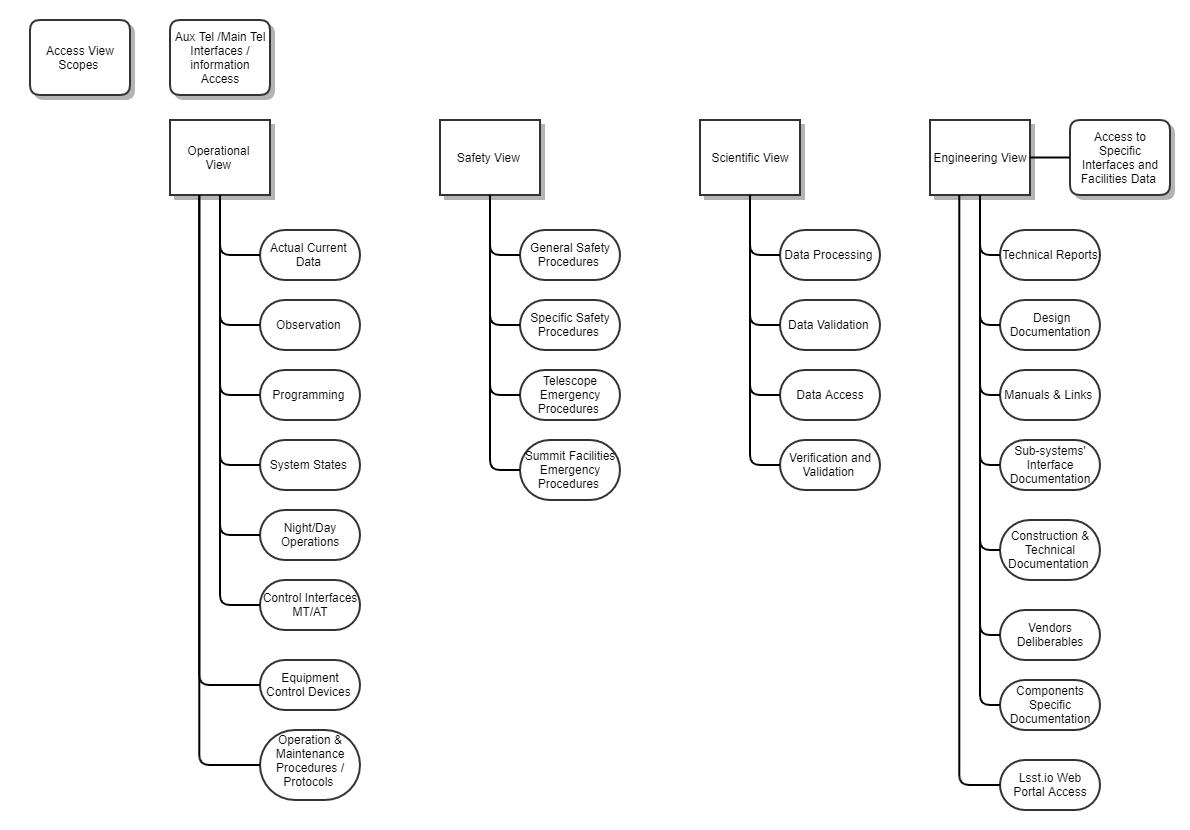
\includegraphics[width=\textwidth]{access-view-example-temp}
\label{fig:access-view-example}
\end{figure}

\subsubsection{Operational View}

Operational View helps with interfaces of real-time data and visualization, observations and its programming, and system state.
It may be natural to separate via leaf-nodes the Main Telescope from the AuxTel to capture specific differences such as control interfaces.
Another natural break down could be day- and night-time operations.
Groups should take advantage of commonalities and referential nature of the Documentation Views.
Users include use of equipment control devices, procedures and protocols for operation and maintenance, such as control room staff, viewing assistants.

\begin{figure}[ht]
\caption{Temporary Caption.}
\centering
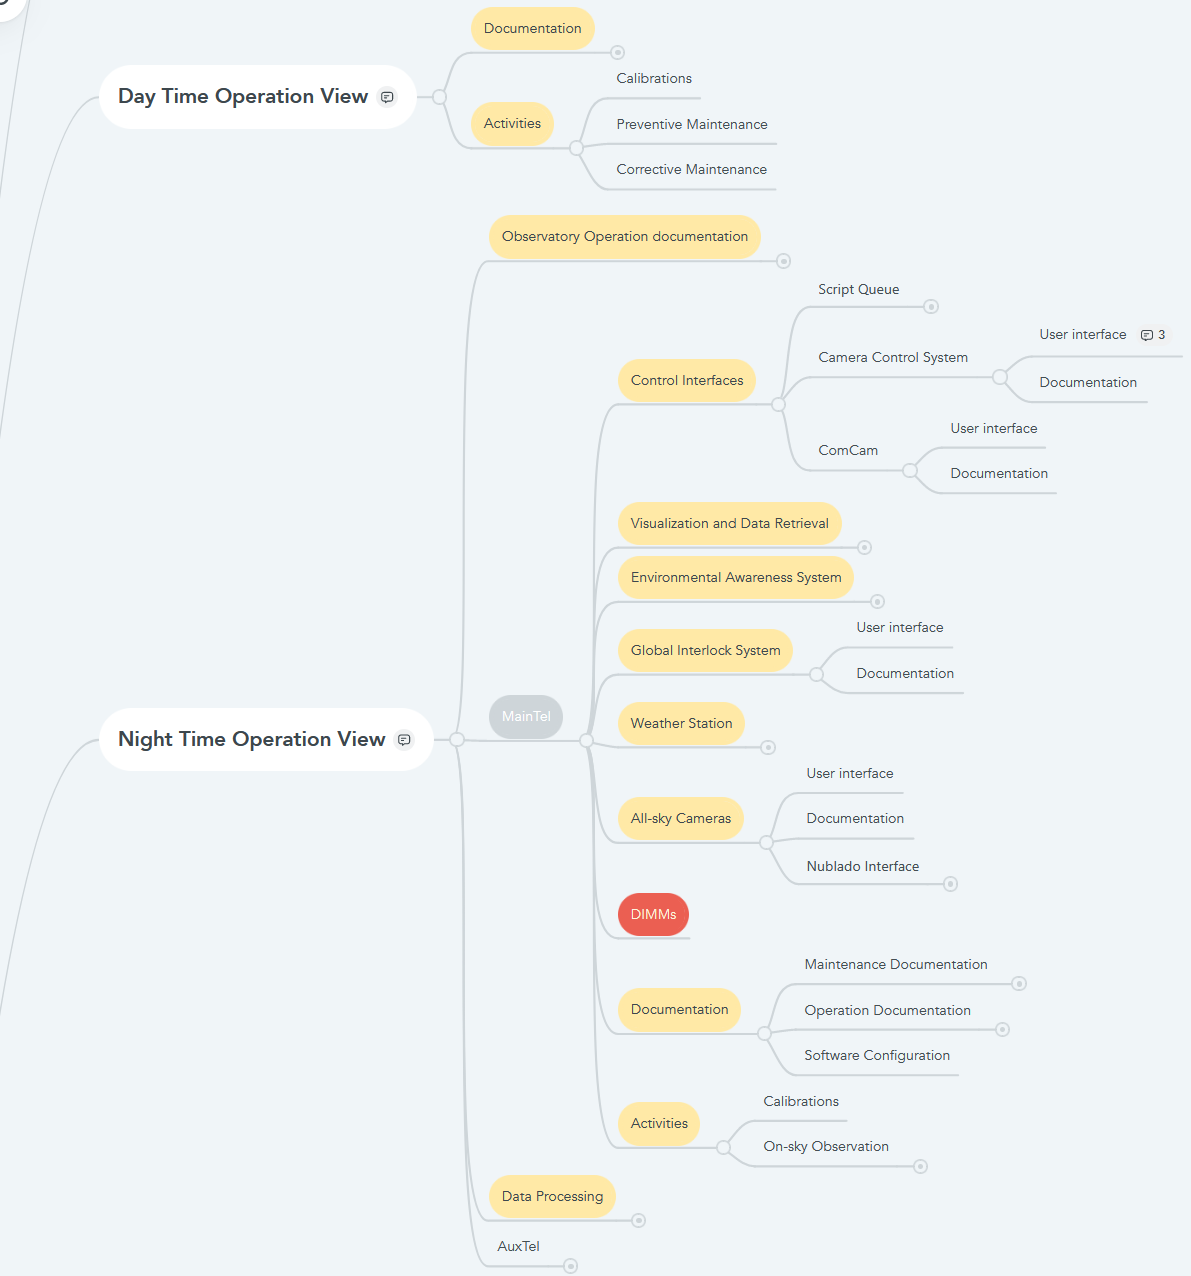
\includegraphics[width=\textwidth]{access-veiw-day-night-operations-example-temp}
\label{fig:access-veiw-day-night-operations-example-temp}
\end{figure}

\subsubsection{Safety View}

The Safety View focuses on accessing the different information related directly to Safety Procedures and Protocols that apply to the different systems.
This can help add consistency and appropriate requirements as necessary.
This Access Would lead users to General Safety procedures, Specific Safety Procedures, Emergency Procedures of telescope and summit facilities.
These Collections shall be available to cover the information needed during activities authorized by the safety and security team

Users include safety, engineering, security, maintenance staffs and management.

\begin{figure}[ht]
\caption{Temporary Caption.}
\centering
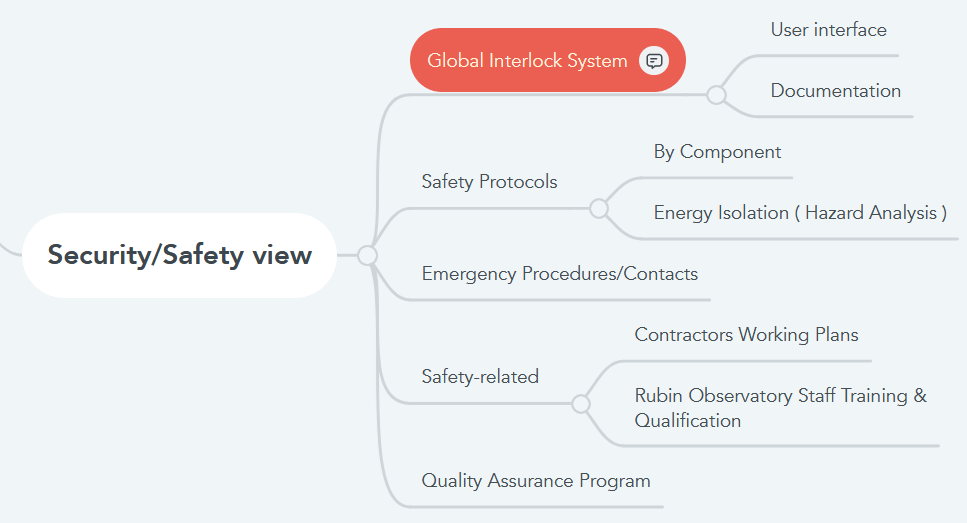
\includegraphics[width=\textwidth]{access-veiw-safety-example-temp}
\label{fig:access-veiw-safety-example-temp}
\end{figure}

\subsubsection{Scientific View}

The Scientific View aims at access to scientific platforms and interfaces that correspond to Rubin Observatory science objectives.

\begin{figure}[ht]
\caption{Temporary Caption.}
\centering
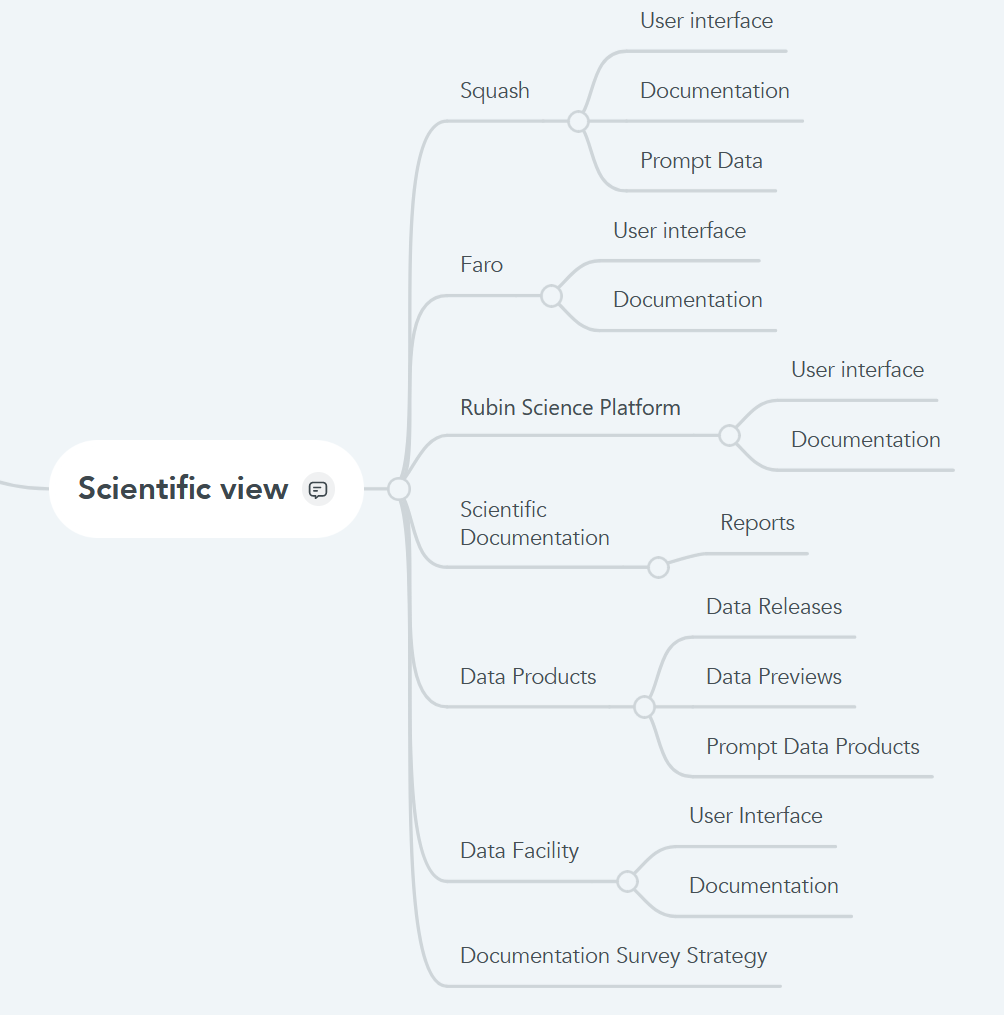
\includegraphics[width=\textwidth]{access-veiw-scientific-example-temp}
\label{fig:access-veiw-scientific-example-temp}
\end{figure}

\subsubsection{Engineering View}

The purpose of the Engineering View is access to Rubin Observatory technical information, including:

\begin{itemize}
\item Accessing specific interfaces and facilities data
\item Sub-systems' Documentation and components to implement an activity 
The Linking access structure would lead users to:
\item Technical Reports
\item Design Documentation
\item Manuals and links to other components documentation
\item Sub-systems' Interface Documentation
\item Construction Documentation. Technical Documentation for the software is separated from hardware Documentation. Technical Documentation within Engineering view:
\item Subsystem Documentation Interfaces
\item Manuals
\item Vendors deliverables
\item Specific documentation by component
\end{itemize}

There are many way and justifications on how to break this view into leaf-nodes.
As the Documentation Working Group developed this, many people readily used a system decomposition as one form.
Other found it potentially useful to break the tree down to specific activity types, e.g., Validation/Verification, Failure Evaluation, Maintenance, Engineering Control, Engineering Design.
Combining these example breakdowns can also be considered.
With such sprawling associated subjects, it's more crucial to develop a strategy to break these leaf-nodes down further by considering categories, impacts to users and how they could want to find associated information.
Note that the Topic View should also be considered when performing this development exercise.
